\documentclass[a4paper,10pt]{article}
\usepackage[utf8]{inputenc}
\usepackage{amsmath}
\usepackage{graphicx}
\usepackage{subcaption}
\usepackage{caption}
\usepackage{hyperref}
\usepackage{float}
\usepackage{epstopdf} 		%Convert EPS files to PDF format
\usepackage{pdfpages} 		%Utility to include pdf documents into the report, used to include datasheets in appendices.
\usepackage{tikz} 			%Utility to draw nice figures
\usepackage{circuitikz} 	%Utility to draw circuits in tikz
\usetikzlibrary{shapes, arrows, chains, scopes, positioning}

\tikzstyle{block} = [draw, fill=blue!20, rectangle, minimum height=3em, minimum width=6em]
\tikzstyle{blockg} = [draw, fill=green!20, rectangle, minimum height=3em, minimum width=6em]

\usepackage{todonotes}
\usepackage{listings}
\usepackage{dcolumn}

\usepackage{fullpage}

\usepackage{xcolor}
\hypersetup{
    colorlinks,
    linkcolor={red!50!black},
    citecolor={blue!50!black},
    urlcolor={blue!80!black}
}

\setlength{\parindent}{0pt}

\title{Drives and Control - DC Motor Speed Control}
\author{Thomas Søndergaard Christensen, Erlingur Ívar Jóhannsson, Mikkel Skarup Jaedicke, Catalin Ionut Ntemkas}
\date{dd/mm/yyyy}


\begin{document}


\begin{titlepage}
\begin{center}

\textsc{\LARGE University of Southern Denmark}\\[1.5cm]
\textsc{\Large MSc in Engineering - Electronics}\\
\textsc{\large Drives and Control}\\[0.5cm]
\vfill
\hrule ~\\[0.3cm]
{ \huge \bfseries DC Motor Speed Control\\[0.4cm] }
\hrule ~\\[1.5cm]
\vfill

% Author and supervisor
\begin{minipage}[t]{.49\textwidth}
\begin{flushleft} \large
\textbf{Author:}\\
ddmmyy Catalin\\
030192 Mikkel Skarup Jaedicke\\
ddmmyy Erlingur Ívar Jóhannsson\\
100589 Thomas S. Christensen
\end{flushleft}
\end{minipage}
\begin{minipage}[t]{.49\textwidth}
\begin{flushright} \large
\textbf{Supervisors:} \\
Jacob Lykke Pedersen\\
\end{flushright}
\end{minipage}

\vspace{1.2cm}
Date: 11-04-2016

\end{center}
\end{titlepage}


\newpage
\tableofcontents
\newpage
\listoffigures
\listoftables
\listoftodos
\clearpage
\newpage
%!TEX root = ../main.tex
\section{Introduction}
\todo[inline]{Do something about list of figures - Thomas}
\todo{Pittmann -> Pittman - Thomas}

Designing a control system for a DC motor is a multi-step process. 
It involves the parametrization of the system, the design of the controller as well as simulations and experiments to determine the best strategy to follow in certain situations depending on the plant. 
The purpose of this report is to go through these steps and provide the reader with the information required in such a procedure. 
Also, this report has been written using the citation \cite{feedback} as the main source of theoretical knowledge. 
The motor models that are used are the Pittman 9234S007-R1 and 9234S006 \cite{pittmann}.
\\

Finding parameters such as the inductance and constants of a motor can be achieved by experimental procedures using appropriate instruments. 
The parameters to be calculated throughout this report are; the voltage constant, the armature resistance, the viscous damping factor, the motor inductance and the inertia. 
In some cases, more than one method is followed for greater accuracy of the data. 
The data is compared with the datasheet of the motors to validate the results. 
The parameters found by experimentation are used in different controllers to drive and test the motor. 
\\

Throughout this report different controller topologies will be utilised, such as a PID and an IPD controller. 
Additionally, the order required to control the motor effectively will be determined. 
The transfer functions will be analysed in order to better understand how they function.
Some work will be done to implement different strategies to improve the behaviour of the overall system, such as noise filtering and anti-windup. 
The design of such systems play an important role in the process of designing a controller. 
The effectiveness of these strategies are not only affected by the environment and the overall system, but also from the settling time, which is an important variable to take into account. 
Lastly, the parameters are inserted in the gain equations of the controllers to receive the gains for a specified system.
\\

After designing a controller, simulations must be run in order to examine how the system behaves under ideal conditions. 
Different controllers will be examined such that the most efficient and suitable one can be chosen for a specific purpose. 
Specifically, the IPD and PI are tested in this report with and without load or extra inertia at different speeds. 
The two controllers are also tested under real conditions using the Pittman motors with the same parameters such as speed and load step that are used under the simulations. 
Finally, the results from the real world and the simulated experiments are compared to each other to observe any similarities or differences at the overall system's behaviour.

\todo{Ensure periods at all captions - Catalin}
\newpage
%!TEX root = ../main.tex
\section{Hardware implementation}
The group was given 2 Pittman 9234 24V motors, the models being 9234S007-R1 and 9234S006, a dual H-bridge and a dSPACE system.
The Pittman 9234S007 is equipped with a rotational encoder.
The dSPACE system is connected to the H-bridge which drives the motors. 
The setup can be seen in figure~\ref{fig:implementation_block}.
Furthermore, the encoders of the motor are connected to the dSPACE system.
A Lecroy wavesurfer 3054 oscilloscope with current probes and KE 34310A multimeters are used in the experiments conducted throughout the report.

\begin{figure}[!h]
\centering
%!TEX root = ../main.tex

%\documentclass{standalone}

%\usepackage{tikz}

% The block diagram code is probably more verbose than necessary
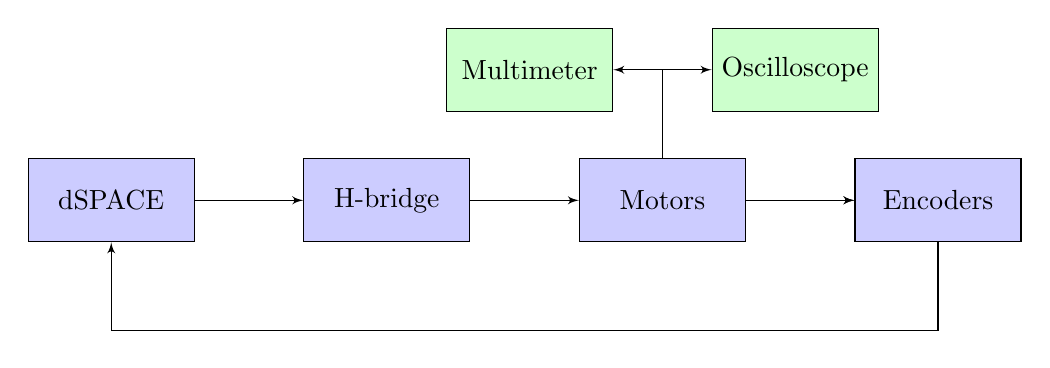
\begin{tikzpicture}[auto, node distance=3.5cm,>=latex']
    % We start by placing the blocks
    \node [block] (motor) {Motors};
    \node [block, left of=motor] (hbro) {H-bridge};
    \node [block, left of=hbro] (dspace) {dSPACE};
    \node [block, right of=motor] (encoder) {Encoders};
    \node [below= 1cm of motor] (point) {};
    \node [above= 1cm of motor] (point1) {};
    \node [blockg, right =0.5cm of point1] (scope) {Oscilloscope};
    \node [blockg, left =0.5cm of point1] (multi) {Multimeter};


    \draw[->] (hbro) -- (motor);
    \draw[->] (dspace) -- (hbro);
    \draw[->] (motor) -- (encoder);
    \draw[->] (motor) -- (encoder);
    \draw[-] (encoder) |- (point.west);
    \draw[->] (point) -| (dspace);
    \draw[->] (motor) |- (scope);
    \draw[->] (motor) |- (multi);


  %\node[label=above:C] (C)  [below right=0.7cm and 4cm of B1]
   %    {($2m-1$)};
    %\draw [draw,->] (input) -- node {$r$} (sum);
    %\draw [->] (sum) -- node {$e$} (controller);
    %\draw [->] (system) -- node [name=y] {$y$}(output);
    %\draw [->] (y) |- (measurements);
\end{tikzpicture}

%\end{document}


  \caption{Block diagram showing the motor setup.}
  \label{fig:implementation_block}
\end{figure}

The dSPACE system was setup with a low sampling time, $T_s$, in order to avoid oversampling the encoder inputs.
$T_s$ and $f_S$ was choosen to be $\frac{1}{1kHz}$ and $25kHz$, respectively. 
The hardware setup of the encoder input and the PWM output can be seen in figure \ref{fig:encoder} and \ref{fig:pwm}, respectively.


\begin{figure}[!h]
\centering
\includegraphics[scale=0.3]{graphics/encoder.png}
  \caption{Encoder setup in dSPACE.}
  \label{fig:encoder}
\end{figure}

\begin{figure}[!h]
\centering
\includegraphics[scale=0.3]{graphics/pwm.png}
  \caption{PWM setup in dSPACE.}
  \label{fig:pwm}
\end{figure}

\newpage
%!TEX root = ../main.tex
\section{Modelling a DC motor}
This section deals with the modelling and parameterisation of a brushed DC motor, specifically the Pittmann 9234 24V servomotor.
Figure \ref{fig:dcmotormodel} is a simple model of a DC motor.
The parameters of this model will be estimated by experimentation.

\begin{figure}[!h]
	\centering
	\includegraphics[width=\linewidth]{graphics/dcmotormodel.png}
	\caption{Simulink model of a brushed DC motor.}
	\label{fig:dcmotormodel}
\end{figure}

For the experiments a test setup is supplied. 
A diagram of the setup can be seen in figure \ref{fig:motorsetup}. 
As can be seen, two motors are connected by the shafts through an external inertia.
The shafts of the two motors will rotate in opposite directions given the same voltage.
To simulate this, a gearbox (called Inverter on the figure) with gear ratio -1:1 is placed between the two motors.
Finally, the Pittmann 9234S007-R1 is equipped with an encoder to allow for monitoring of the angular velocity of the shaft.


\begin{figure}[!h]
	\centering
	\includegraphics[width=.8\linewidth]{graphics/motorsetup.png}
	\caption{Simulink model of the motor setup provided for the project.}
	\label{fig:motorsetup}
\end{figure}

\subsection{Voltage Constant - $K_e$}
\label{sec:voltconstat}
The voltage constant describes the relationship between applied voltage and the resulting angular velocity of the rotor:
\begin{equation}
	\label{eq:voltconstant}
	K_e\omega_r = V_{cc}
\end{equation}
where $\omega_r$ is the angular velocity of the rotor and $V_{cc}$ is the voltage across the motor.
From equation \ref{eq:voltconstant} it is apparent that $K_e$ can be determined if the voltage across the terminals of the motor is measured while the motor is being run at a known velocity.
The experiment is conducted as follows:
A voltage is applied across the terminals of the Pittmann 9234S006.
The resulting velocity of the assembly is monitored using the encoder on the Pittmann 9234S007.
Across the terminals of this motor is now only the back-EMF.
This value is recorded.
Figure \ref{fig:velvsvolt} shows the recorded data. 
As is expected, there is a highly linear relationship between the voltage and velocity.
The final value of $K_e$ is determined by averaging and then dividing the collected data.
$$K_e=\frac{V_{cc}}{\omega_r}=0.0360$$
This value is within 1.2\% of the value given in the datasheet \cite{pittmann}.

\begin{figure}[!h]
	\centering
	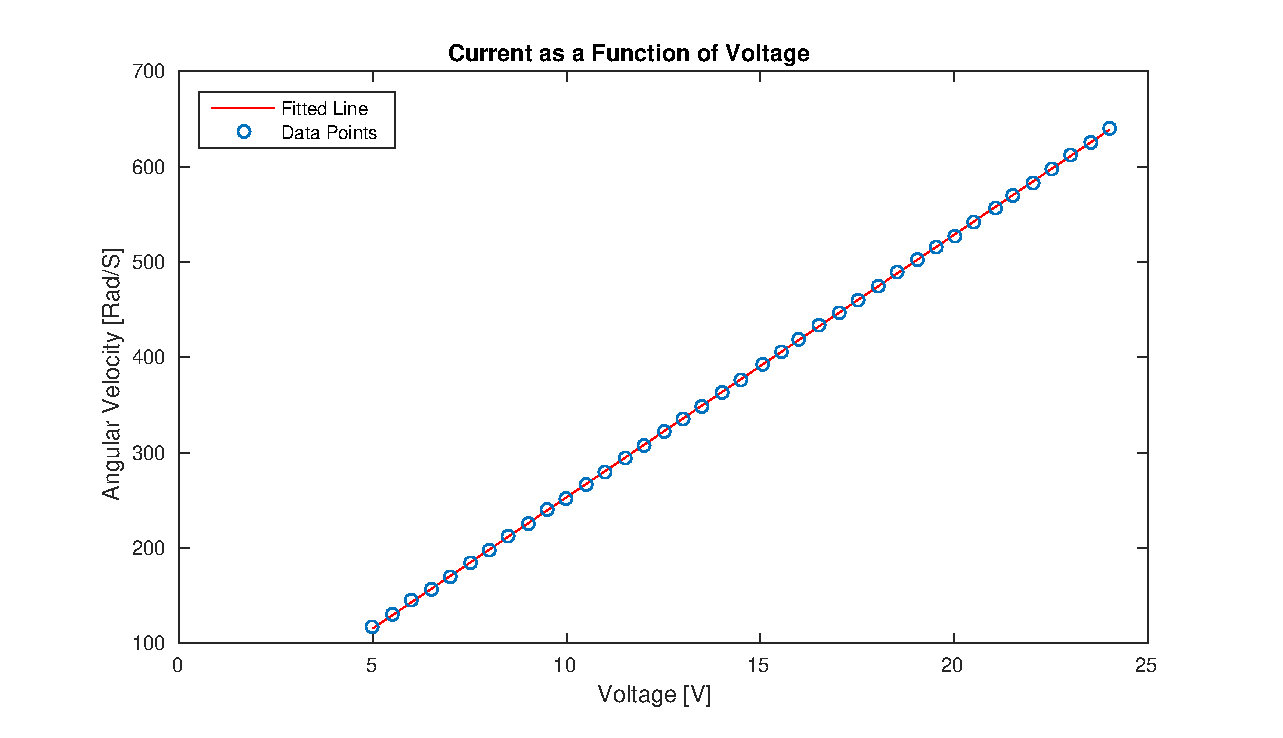
\includegraphics[width=\linewidth]{graphics/vvsrpm}
	\caption{Angular velocity of the shaft at different voltages.}
	\label{fig:velvsvolt}
\end{figure}

\subsection{Armature Resistance - $R_a$}
\paragraph{Method 1:}~\\
The armature resistance, $R_a$ in figure \ref{fig:dcmotormodel}, can be found simply by applying Ohm's law.
The current through a resistor is well defined when a voltage is applied across it.

\begin{figure}[!h]
	\centering
	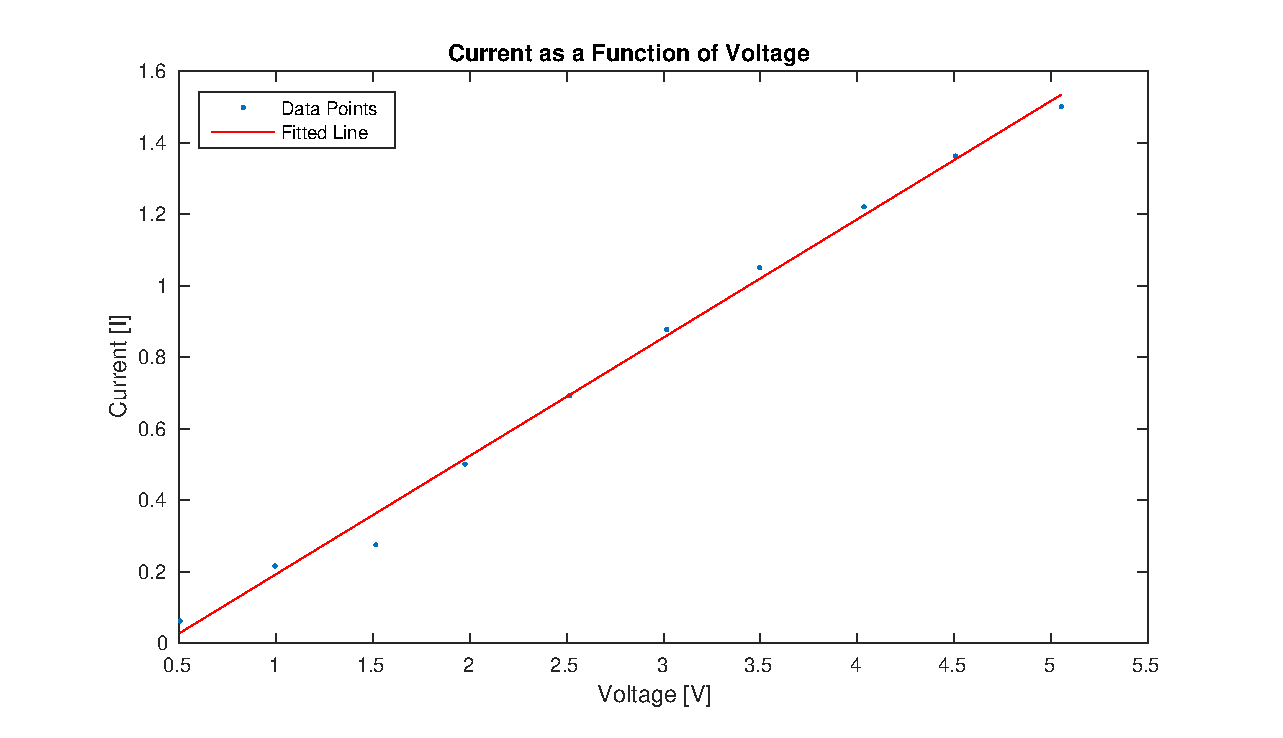
\includegraphics[width=\linewidth]{graphics/raplot}
	\caption{Current as a function of voltage with the rotor blocked.}
	\label{fig:raplot}
\end{figure}

However, when the rotor is spinning, the circuit produces back-EMF.
This counters the input voltage, effectively lowering the current through $R_a$.
In order to avoid this effect the rotor is blocked.
Since, with a blocked rotor, there will be no change in voltage in the system, the inductor acts as a short circuit, reducing the circuit to a voltage across a resistor. 

Figure \ref{fig:raplot} shows the data collected in order to determine the value of the armature resistance.
A voltage is applied across the terminals at 0.5 V.
According to the datasheet \cite{pittmann} the current at maximum allowed continuous torque is 1.75 A.
This current is reached at 5 V, therefore, the measurements stop there.
As can be seen from the figure, a line is fitted to the data.
This is done using the linear least squares method with the following result:
$$I(V)=0.272\cdot V-0.042$$
with $R^2=0.995$.
Since for the plot $I(V)$:
$$R_a = \frac{1}{\text{slope}} = 3.683\Omega$$
This value is significantly higher, approximately 25\% higher, than the value given in the datasheet.
Additionally, the final data points seem to become irregular.
This is likely caused by the high currents drawn by the motor at these voltages warming the motor and therefore slightly altering the characteristics of the resistor.

For these reasons it has been decided to pursue a different means of determining the armature resistance:
\paragraph{Method 2}~\\
This method makes use of the voltage constant found in section \ref{sec:voltconstat}.
By expanding $V_cc$ in equation \ref{eq:voltconstant} an expression for $R_a$ can be found:
\begin{equation}
	\label{eq:voltconstantexpanded}
	K_e\omega_r = V_{cc} = I_aR_a\quad \Rightarrow \quad R_a = \frac{\omega_rK_e}{I_a}
\end{equation}
Similarly to the experiment in section \ref{sec:voltconstat}, one motor is used to spin the other to speed.
This time, however, the terminals of the Pittmann 9234S007 are connected through a power resistor, $R_e$.
Obviously then:

\begin{eqnarray}
	R_t =& R_a + R_e\\
	R_a =& \frac{\omega_rK_e}{I_a}-R_e
\end{eqnarray}

where $R_t$ is the total resistance in the system.
As the voltage across the terminals of the Pittmann 9234S006 is increased the resulting velocity and current is noted.
Finally, the armature resistance is found to be:
$$R_a = 3.715\Omega$$

\newpage
\section{Controlling}

\todo{PUT DOTS AT the end of figures' sentences}

To control the speed of the DC motor a controller will have to be implemented in to the system. A block diagram of the DC motor in figure~\ref{fig:dcmotormodel} is shown in figure~\ref{fig:dcblock}. From the block diagram a transfer function $P(s)$ for the motor can be derived as seen in equation~\ref{eq:fullplant} on the form in equation~\ref{eq:simpleplant}.

\begin{figure}[!h]
	\centering
	\includegraphics[width=.75\linewidth]{graphics/dcblockdiagram}
	\caption{A block diagram of the DC motor}
	\label{fig:dcblock}
\end{figure}


\begin{equation}
\label{eq:fullplant}
P(s) = \dfrac{\dfrac{K_m}{J_r L_a}}{s^2 + \dfrac{J_r R_a + L_a T_{fv}}{J_r L_a}s + \dfrac{R_a T_{fv} +K_m^2}{J_r L_a}}
\end{equation}

\begin{equation}
\label{eq:simpleplant}
P(s) = \dfrac{b_0}{s^2 + a_1 s + a_0}
\end{equation}


\subsection{PID controller}
 A commonly used controller is the PID controller\cite{feedback}. The name comes from its three adjustable parameters, the proportional gain $K_{P}$, integral gain $K_{I}$ and the derivative gain $K_{D}$. Reason for its popularity is the wide range of operating conditions as well being relatively easy to understand. 
 
 The controller is placed at the input of the motor monitoring the output through a feedback. the system is shown in figure~\ref{fig:pidcontrolsystem} where the plant is the DC motor. The transfer function $H(s)$ of the system is shown in equation~\ref{eq:tfpidsystem} where $C(s)$ is the transfer function of the controller.

\begin{figure}[!h]
	\centering
	\includegraphics[width=.75\linewidth]{graphics/controlsystem}
	\caption{Block diagram of the PID control system}
	\label{fig:pidcontrolsystem}	
\end{figure}

\begin{equation}
\label{eq:tfpidsystem}
H(s) = \dfrac{C(s)P(s)}{1+C(s)P(s)}
\end{equation}

A block diagram for the PID controller can be seen in figure~\ref{fig:pidblock} and its transfer function in equation~\ref{eq:pid}.  

\begin{figure}[!h]
	\centering
	\includegraphics[width=.7\linewidth]{graphics/pidcontroller}
	\caption{Block diagram of the PID-controller}
	\label{fig:pidblock}
\end{figure}

\begin{equation}
\label{eq:pid}
C(s) = K_P + \dfrac{K_I}{s} +K_D s
\end{equation}

Inserting the transfer functions $C(s)$ and $P(S)$ into the transfer function $H(s)$ and rearranging it, $H(s)$ becomes the equation~\ref{eq:pidfulltf}. On the new form, the denominator describes the poles of the system and is called the characteristic equation.

\begin{equation}
\label{eq:pidfulltf}
H(s) = \dfrac{b_0 (K_D s^2 + K_P s K_I)}{s^3 + (a_1 + b_0 K_D)s^2 (a_0 + b_0 K_P)s + b_0 K_I }
\end{equation}


\subsection{IPD controller}
An equivalent setup to the PID controller is the IPD controller, which does not introduce zeros to the system. It still uses the same gains (proportional, integral and derivative gain) and due to its design, eliminates overshoots as well as undershoots.

\begin{figure}[!h]
	\centering
	\includegraphics[width=.85\linewidth]{graphics/ipdcontroller}
	\caption{Block diagram of the IPD control system}
	\label{fig:ipdcontrolsystem}	
\end{figure}

Due to no zeros to the overall system, the transfer function of the IPD controller system becomes as seen in the equation~\ref{eq:tfipdsystem}.

\begin{equation}
\label{eq:tfipdsystem}
H(s) = \dfrac{\dfrac{K_I}{s} P(s)}{1+C(s)P(s)}
\end{equation}

With insertion and rearranging, the transfer function $H(s)$ takes the form of equation~\ref{eq:ipdfulltf}. Now it can be seen that indeed the IPD controller does not introduce any zeros to the system and the characteristic equation is same as the one for the PID controller. Thus the same controller gains can be used in both cases.

\begin{equation}
\label{eq:ipdfulltf}
H(s) = \dfrac{b_0 K_I}{s^3 + (a_1 + b_0 K_D)s^2 (a_0 + b_0 K_P)s + b_0 K_I }
\end{equation}

\subsection{Noise Filtering}

The derivative part of the PID controller will try to reduce every sudden change in the system. This is what helps the system stop oscillating. However, when noise is introduced to the system, the derivative term acts on the fast, sudden change and can destabilize the system. In other words, the derivative term can and will increase the noise. For this reasons a low pass filter is needed on the derivative path. This is done with changing $s$ on the derivative gain to $N/(s + N)$ where $N$ is $1/T_f$ and $T_f$ is the filter time constant and N is the cut off frequency. The block diagram for the controllers then become as seen in figures~\ref{fig:pidfilter} and~\ref{fig:ipdfilter} respectively.

\begin{figure}[!h]
	\centering
	\includegraphics[width=.7\linewidth]{graphics/pidwfilter}
	\caption{Block diagram of the PID controller with filter}
	\label{fig:pidfilter}
\end{figure}

\begin{figure}[!h]
	\centering
	\includegraphics[width=.9\linewidth]{graphics/ipdwfilter}
	\caption{Block diagram of the IPD controller with filter}
	\label{fig:ipdfilter}
\end{figure}


\subsection{Anti-Windup Design}

During the function of the controller, there is a possibility that it will operate in a nonlinear region where increasing the control signal has no effect on the system output. This introduces time delay to the response of the system, thus reducing its overall performance. This behaviour can be counteracted using an anti-windup strategy such as the one in figure~\ref{fig:ipdantiwindupstrategy}.

\begin{figure}[!h]
	\centering
	\includegraphics[width=.9\linewidth]{graphics/ipdwindupdesign}
	\caption{Block diagram of the IPD controller with anti-windup strategy}
	\label{fig:ipdantiwindupstrategy}
\end{figure}

As figure~\ref{fig:antiwindupresponses} shows, using this strategy introduces smoother behaviour into the system. The gain $K$ is the one that determines that behaviour and can be chosen doing experiments using trial and error. An interesting observation is that the value of $K$ for the PID controller is quite different from the one for the IPD controller. Specifically, a suitable value for PID is $K=10$, while for IPD is $K=10000$. That conclusion has been reached through experiments, and the results can be seen in the figure~\ref{fig:pidwindupvaluecomp}.

One major disadvantage of implementing such a strategy is that the settling time suffers for low values such as $T_s=0.01$, but not for $T_s=0.1$ as it can be seen in figure. 
\todo{update the windup resonse graphs!}
\begin{figure}
	\centering
	\begin{subfigure}[b]{0.45\textwidth}
		\includegraphics[width=\textwidth]{graphics/pidwindupresponse}
		\caption{PID controller}
		\label{fig:pidwindupresponse}
	\end{subfigure}
	~ %add desired spacing between images, e. g. ~, \quad, \qquad, \hfill etc. 
	%(or a blank line to force the subfigure onto a new line)
	\begin{subfigure}[b]{0.45\textwidth}
		\includegraphics[width=\textwidth]{graphics/ipdwindupresponse}
		\caption{IPD controller}
		\label{fig:ipdwindupresponse}
	\end{subfigure}
	\caption{Responses of controllers without (yellow line) and with (blue line) anti-windup strategy.}\label{fig:antiwindupresponses}
\end{figure}


\begin{figure}[!h]
	\centering
	\includegraphics[width=.75\linewidth]{graphics/pidwindupvaluecomp}
	\caption{PID behaviour with different anti-windup gain: 10000 (blue line) and 10 (yellow line).}
	\label{fig:pidwindupvaluecomp}
\end{figure}

\subsection{Controller Gain Design}

\subsubsection{Settling Time Formula}

The equation~\ref{eq:settling} is used for the desired response to enter the 5$\%$ error band within the given settling time.
\begin{equation}
\centering
\label{eq:settling}
\alpha = \dfrac{1.5(1 + n)}{T_s}
\end{equation}

\begin{table}[!h]
	\caption{ Coefficients of
		closed loop differential
		equation based on settling
		time formula\cite{feedback}}
	\centering
	\begin{tabular}{|c|c|c|c|}
		\hline
		n & 2 & 3 & 4\\
		\hline
		$d_0$ & $\alpha^2$ & $\alpha^3$ & $\alpha^4$\\ 
		$d_1$ & $2\alpha$ & $3\alpha^2$ & $4\alpha^3$\\
		$d_2$ & - & $3\alpha$ & $6\alpha^2$\\
		$d_0$ & - & - & $4\alpha$\\
		\hline	
		
	\end{tabular}
	\label{table:coefsettlingtime}
\end{table}


\subsubsection{Full Order Systems}

As the equations~\ref{eq:pidfulltf} and~\ref{eq:ipdfulltf} show, their denominator is in the standard form~\ref{eq:stdchararacteristic}. The coefficients from the characteristic equations can easily be matched with the ones from the standard form as shown in~\ref{eq:pidmatchingcoef} together with the coefficients table~\ref{table:coefsettlingtime} where the order of the system in this case is $n=3$.


\begin{equation}
\centering
\label{eq:stdchararacteristic}
s^n + d_{n-1}s^{n-1} + \cdots + d_1 s + d_0 
\end{equation}

\begin{align}
\label{eq:pidmatchingcoef}
d_0 &= b_0 K_I = \alpha^3
\\
d_1 &= a_0 + b_0 K_P = 3\alpha^2
\\
d_2 &= a_1 + b_0 K_D = 3\alpha
\end{align}

Solving the above equations using the parameters and $T_s=10ms$, the gains receive the values:
\begin{align*}
\label{eq:gainsvaluesfull}
K_I &= 62.3855
\\
K_P &= 0.2752
\\
K_D &= 1.7910\cdot10^{-4}
\end{align*}


\subsubsection{Reduced Order Systems}

In the case of a reduced order system, the controller derivative's gain is equal to zero, and the transfer function takes the form of equation~\ref{eq:pireducedtf}.

\begin{equation}
\label{eq:pireducedtf}
H(s) = \dfrac{b_0(K_Ps + K_I)}{s^2 + (a_0 + b_0 K_P)s + b_0 K_I }
\end{equation}

Matching the characteristic equation with the standard form and looking at the table~\ref{table:coefsettlingtime}, the coefficients become:

\begin{align*}
\label{eq:pimatchingcoef}
d_0 &= b_0 K_I = \alpha^2
\\
d_1 &= a_0 + b_0 K_P = 2\alpha
\end{align*}

Similarly, using the parameters and $T_s=10ms$, the gains in this case are:

\todo{calculate the gains here too!}


\newpage
\section{Simulations}
Before the controllers can be tested on the real system a simulation must be done. The controllers that have been chosen are the IPD and PI, where PI is the PID controller with $K_D$ set to 0. Speed control is simulated at two different angular velocities, 200~rad/s and~125 rad/s To prevent the saturation limit to be reached, the settling time is set to 0.1~ms.\todo{why settling time 0.1 and not 0.01}

\begin{figure}[h!]
	\centering
	\begin{subfigure}[b]{0.45\textwidth}
		\includegraphics[width=\textwidth]{graphics/PI_single125}
		\caption{PI Speed control at 125 rad/s}
		\label{fig:pisingle125}
	\end{subfigure}
	~ %add desired spacing between images, e. g. ~, \quad, \qquad, \hfill etc. 
	%(or a blank line to force the subfigure onto a new line)
	\begin{subfigure}[b]{0.45\textwidth}
		\includegraphics[width=\textwidth]{graphics/PI_single200}
		\caption{PI Speed control at 200 rad/s}
		\label{fig:pisingle200}
	\end{subfigure}
	\caption{The PI controller at two different angular velocities. It is noticed that the desired settling time is reached in both cases.}\label{fig:pisingle}
\end{figure}






\begin{figure}[h!]
	\centering
	\begin{subfigure}[b]{0.45\textwidth}
		\includegraphics[width=\textwidth]{graphics/IPD_single125}
		\caption{IPD Speed control at 125 rad/s}
		\label{fig:ipdsingle125}
	\end{subfigure}
	~ %add desired spacing between images, e. g. ~, \quad, \qquad, \hfill etc. 
	%(or a blank line to force the subfigure onto a new line)
	\begin{subfigure}[b]{0.45\textwidth}
		\includegraphics[width=\textwidth]{graphics/IPD_single200}
		\caption{IPD Speed control at 200 rad/s}
		\label{fig:ipdsingle200}
	\end{subfigure}
	\caption{The PI controller at two different angular velocities. A delay is introduced. The desired settling time is reached from when the controller responses.}\label{fig:ipdsingle}
\end{figure}



The simulation confirms that the controllers behave similar for both simulated angular velocities as seen in figures~\ref{fig:pisingle} and~\ref{fig:ipdsingle}. The settling time reaches the desired value for both PI and IPD. However an unexplained delay is introduced in the beginning of the IPD controller response. That delay does not affect the system response in other way than offsetting it.

\begin{figure}[h!]
	\centering
	\begin{subfigure}[b]{0.45\textwidth}
		\includegraphics[width=\textwidth]{graphics/PI_load125}
		\caption{PI Speed control at 125 rad/s}
		\label{fig:piload125}
	\end{subfigure}
	~ %add desired spacing between images, e. g. ~, \quad, \qquad, \hfill etc. 
	%(or a blank line to force the subfigure onto a new line)
	\begin{subfigure}[b]{0.45\textwidth}
		\includegraphics[width=\textwidth]{graphics/PI_load200}
		\caption{PI Speed control at 200 rad/s}
		\label{fig:piload200}
	\end{subfigure}
	\caption{The PI controller at two different angular velocities with added load. Desired settling time is not reached. Instead it introduces an overshoot and does not become stable until it is close to 1s.}
	\label{fig:piload}
\end{figure}

\begin{figure}[h!]
	\centering
	\begin{subfigure}[b]{0.45\textwidth}
		\includegraphics[width=\textwidth]{graphics/IPD_load125}
		\caption{IPD Speed control at 125 rad/s}
		\label{fig:ipdload125}
	\end{subfigure}
	~ %add desired spacing between images, e. g. ~, \quad, \qquad, \hfill etc. 
	%(or a blank line to force the subfigure onto a new line)
	\begin{subfigure}[b]{0.45\textwidth}
		\includegraphics[width=\textwidth]{graphics/IPD_load200}
		\caption{IPD Speed control at 200 rad/s}
		\label{fig:ipdload200}
	\end{subfigure}
	\caption{The PI controller at two different angular velocities with added load. The desired settling time is far from being reached. The system becomes stable at around 13s.}
	\label{fig:ipdload}
\end{figure}

When the system has reached the stable output a load step is introduced.
When the load step is added, the IPD controller seems to have a hard time to settle, Figure~\ref{fig:ipdload}. The systems does not reach the stable condition until after 13s. This result could have been estimated thus the controllers were designed with only a single motor in mind. Added load changes the system behaviour and should be controlled with different controller gains.\todo{Catalin: I don't understand the sentence "This result...mind"}

\newpage
\input{bib}

\end{document}

